\documentclass[12pt,oneside]{book}
\pagestyle{headings}

% Note that the line below could be modified to suit a
% particular system since the "geometry" package behaves
% differently in Unix, Windows and Mac, especially for the
% top margins.
% Adjust the parameter "top" (measuring the height of the
% space allocated to a header) and "headsep" (measuring
% the distance from the bottom of the header to the
% first line of text.
\usepackage[top=1.3in,left=1.5in,bottom=1in,right=1in,headsep=0.5in]{geometry}

\usepackage{setspace}
\onehalfspacing
%\doublespacing

% Headers and footers for thesis
\usepackage{fancyhdr}

\markboth{}{}
\newcommand\startchapter[1]{\chapter{#1}\thispagestyle{myheadings}}
\newcommand\startappendix[1]{\chapter{#1}\thispagestyle{myheadings}}
\newcommand\startfirstchapter[1]{\chapter{#1}}

% Manual addition of section to Table of Contents
\newcommand\TOCadd[1]{\newpage\phantomsection\addcontentsline{toc}{chapter}{#1}}

% Float Customization
\renewcommand{\floatpagefraction}{0.01}

% Customization of Tables of Contents and List of Figures/Tables
\usepackage{tocloft}
\renewcommand\cfttabpresnum{Table\ }
\renewcommand\cfttabnumwidth{0.75in}
\renewcommand\cftfigpresnum{Figure\ }
\renewcommand\cftfignumwidth{0.80in}
\newcommand{\HRule}{\rule{\linewidth}{0.5mm}}


% Long Table and decimal aligned columns
\usepackage{dcolumn}
\usepackage{longtable}

% Mathematics support
\usepackage{amsmath}
\delimitershortfall-1sp
\newcommand\abs[1]{\left|#1\right|}

\usepackage{amsthm}
\usepackage{amssymb}


% Text Control
\usepackage{xspace}
\usepackage{textcase}

% Graphics
\usepackage{wasysym}
\usepackage{graphics}
\usepackage{graphicx}   % A package to allow insertion of
                        % external image files
\graphicspath{{Figures/}}
\usepackage[caption=false]{subfig}
\captionsetup{belowskip=8pt,aboveskip=8pt}
\usepackage{multirow}
\newtheorem{remark}{Remark}
\usepackage{algorithmic}
\usepackage[ruled]{algorithm2e}
%\usepackage{epsfig}
\usepackage{epstopdf}
\usepackage{tikz}
%\usepackage{gantt}
\usepackage{titling,enumitem}
\usepackage{url}
\usepackage{makecell}
\usepackage{lscape}
\usepackage{cite}
\usepackage{nomencl}
\makenomenclature
\makeatletter
\def\thenomenclature{%
  \section*{\nomname}
  \if@intoc\addcontentsline{toc}{section}{\nomname}\fi%
  \nompreamble
  \list{}{%
    \labelwidth\nom@tempdim
    \leftmargin\labelwidth
    \advance\leftmargin\labelsep
    \itemsep\nomitemsep
    \let\makelabel\nomlabel}}
\makeatother


% Widecheck
\makeatletter
\DeclareRobustCommand\widecheck[1]{{\mathpalette\@widecheck{#1}}}
\def\@widecheck#1#2{%
    \setbox\z@\hbox{\m@th$#1#2$}%
    \setbox\tw@\hbox{\m@th$#1%
       \widehat{%
          \vrule\@width\z@\@height\ht\z@
          \vrule\@height\z@\@width\wd\z@}$}%
    \dp\tw@-\ht\z@
    \@tempdima\ht\z@ \advance\@tempdima2\ht\tw@ \divide\@tempdima\thr@@
    \setbox\tw@\hbox{%
       \raise\@tempdima\hbox{\scalebox{1}[-1]{\lower\@tempdima\box
\tw@}}}%
    {\ooalign{\box\tw@ \cr \box\z@}}}
\makeatother

\newcommand{\specialcell}[2][c]{%
  \begin{tabular}[#1]{@{}c@{}}#2\end{tabular}}
\makeatletter
\providecommand{\keywords}[1]{\textbf{Index terms---} #1}
\begin{document}
%/////////////////////////////////////////////////////////////////////////////////////////////////////////////////////
\startchapter{A Prediction Model}
\label{chap:predictionModel}
\section{Motivation}
As discussed in Chapter~\ref{chapter:introduction}, the main objective of this work is to increase the reliability of power networks in terms of power quality within given financial budget/resources. In order to monitor the power quality, power quality meters are being deployed. Since power quality meters are expensive devices, we (in chapter~\ref{chap:PQEstimation}) proposed MaxEnt based algorithm for power quality estimation on unmonitored network segments. For meter placements, we proposed conditional entropy based efficient algorithms (in chapter~{chap:meterPlacement}) that intelligently place power meters on selected network segments so that the power quality could be inferred as accurately as possible.

Since the power quality readings (exact readings from monitored links, and estimated PQ values from unmonitored links) are available now, we use these readings to estimate the state of the network and identify any potential malfunctioning device in the power network. Our objective in this chapter is to address the research challenge: \textit{how to detect a potential malfunctioning device in the power network based on available power quality readings}. In the next section, we propose an algorithm that helps to detect the malfunctioning devices in the power network.

\section{Problem Formulation}
\subsection{Assumptions}
We make below assumptions about the problem:
\begin{enumerate}
\item \textit{The transfer function or behavior $\left(f\left(d\right)\right)$ of each device $d$ in the network is known}. As discussed earlier, a device-specific power quality transfer function could be estimated through physical modeling or through the assessment of historical PQ data. In Chapter~\ref{chap:latentF}, using a real power quality dataset, we have shown how accurately an $f(d)$ could be estimated.

\item \textit{All potential malfunction devices need to be on a monitored segment.} A potential malfunction device could effectively be detected when the device itself or any of its child device is monitored in real time using a PQ meter. This assumption is realistic in the sense that if the underline link is not monitored, we cannot get the real-time status of PQ values and would not be able to detect if a device is not behaving normally. The idea is to detect if a device is significantly deviating form its normal behavior.

\item \textit{The power grid network is a tree-structured network where the electric current flows from root node to the child nodes.} Note that this is a reasonable assumption at any particular instance in time. While enterprise level power grids used in places such as hospitals and data centers often have two utility feeds available as well as an independent emergency power source, only one power source is typically used at one time. See the IEEE Gold Book~\cite{goldbook} for further information on recommended practices in the design of critical power systems.

\item \textit{The probability mass function} (\textit{pmf}$\left(d_0\right)$)\textit{ of power quality values at the input link to the root node is known.} In other words, the distribution of power quality at the input to the network, usually the utility feed, is known. This is also a reasonable assumption, since electrical utilities typically report on indices such as System Average RMS Variation Frequency Index (SARFI) which is essentially a count of the number of times the magnitude and duration falls below a threshold. Furthermore, there are often independent bodies that gather statistics on power delivery service reliability that can also be incorporated into an estimate of power quality distribution~\cite{chowdhury2004reliability}.
\end{enumerate}

\subsection{The Problem}
We now formalize the problem of detecting a malfunction device in the network. The objective is to detect a device $d$ in the network as a malfunction device when its power quality output degrades persistently from its normal behavior. Since the transition function $f(d)$ of each device $d$ is known, we know the probability distribution of the output power quality (\emph{pmf}$\left(d\right)$) at the output of each device in the network. Figure 3 shows the probability distributions    any variation $\delta_d$ from $f(d)$ need to be detected and classified. model is     

If no smart meter installed on that device, need to estimate from neighboring links

- The metered link detects deviation and estimate the deviations of all devices between itself and parent metered link


\section{Our Prediction Algorithm}
for every sample -> check if f(d) varies by f1(d)\\
for the detected segment, use maxent to estimate f(d1) to f(dn)\\
sort them by descending order of variation\\
the top one is high probable.

bad power quality events\\
unit time interval\\
window size\\
an interval is bad quality interval when it is classified as >= 4\\
threshold number of bad quality intervals\\
misbehaving device on the detected link\\
candidate links are\\
use maxent


using input pdf simulation dataset was generated\\
we use f(d) as in chapter 3

\begin{figure}[!t]
\centering
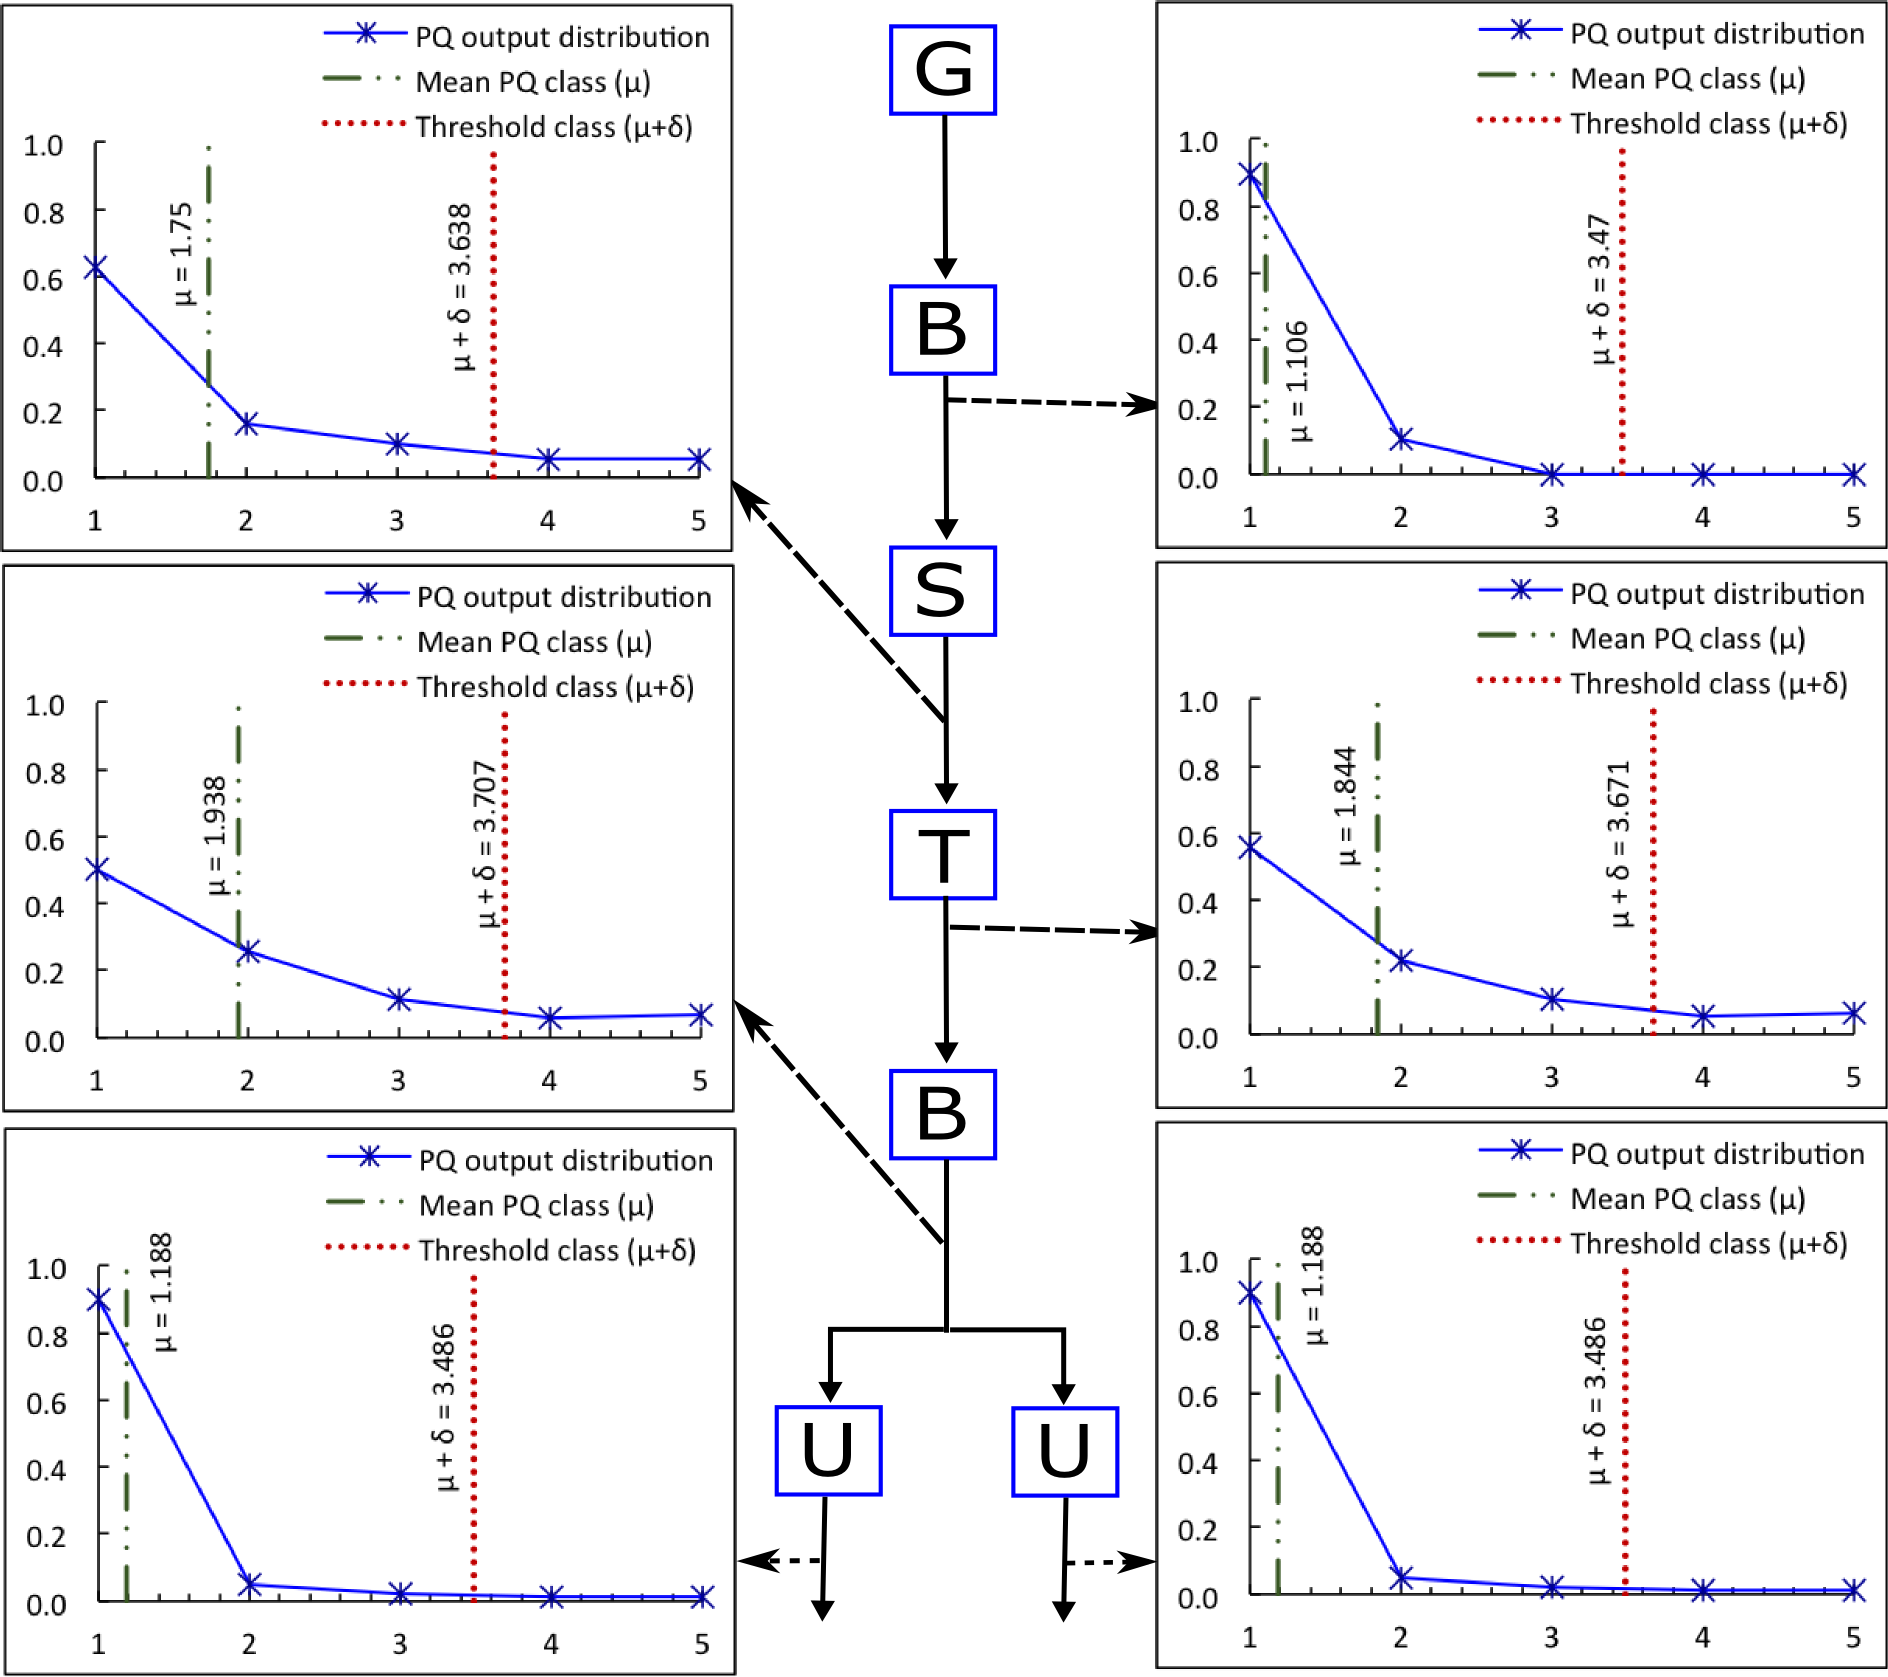
\includegraphics[width=0.98\textwidth]{PQOutputDistribution}
\caption{Power quality distributions at the output links of various devices. The average power quality class and computed threshold is shown as vertical lines in each  distribution graph.}
\label{fig:outputPQDistributions}
\end{figure}

\section{Evaluations}
Assume that one or more smart meters have continuously measured poor power quality. The power quality is indicated by some specific power quality index, for instance the System Average RMS Variation Frequency (SARFI) index . Based on the measured and estimated PQ values, we would like to know which device is most likely to be malfunctioning. Here, we assume that we know the transform function of each device if the device is working properly. We call these transfer functions the regular transform functions of the devices. Now, a malfunctioning device is the one whose estimated transform function deviates significantly from its regular transform function.

We plan to first give a comprehensive mathematical model of the problem. We then device a mechanism to calculate the deviation in transfer functions and finally we plan to propose an algorithm to efficiently identify any potential malfunctioning device in the power network. The proposed algorithm will be evaluated on various tree and bus structured network; specifically we will use the IEEE standard test networks for our simulations.

\section{Conclusion}
Power quality meters play an important role in the reliability of power networks. We plan to investigate the problem of identifying devices that degrade the power quality in the system. The proposed solution will be built on top of our already proposed work.


%/////////////////////////////////////////////////////////////////////////////////////////////////////////////////////
\end{document}